% ~~~~~~~~~~~~~~~~~~~~~~~~~~~~~~~~~~~~~~~~~~~~~~~~~~~~~~~~~~~~~~~~~ %
\newif\ifshownotes													%
\shownotestrue														%
\documentclass{article}
\usepackage[margin = 2cm]{geometry}
\usepackage[english]{babel}
\usepackage[utf8]{inputenc}
\usepackage[T1]{fontenc}
\usepackage{xcolor}
\usepackage{booktabs}
\usepackage{acronym}
\usepackage{listings}
\usepackage[hidelinks]{hyperref}
\usepackage{amsthm}
\usepackage{graphicx}
\theoremstyle{definition}
\newtheorem{example}{Example}[section]
\graphicspath{{../Images/}}

\usepackage{tikz} % ------------------------------- %
\usetikzlibrary{arrows}								%
\usetikzlibrary{calc}								%
\usetikzlibrary{decorations.footprints}				%
\usetikzlibrary{decorations.pathmorphing}			%
\usetikzlibrary{decorations.text}					%
\usetikzlibrary{fadings}							%
\usetikzlibrary{fit}								%
\usetikzlibrary{intersections}						%
\usetikzlibrary{matrix}								%
\usetikzlibrary{mindmap}							%
\usetikzlibrary{patterns}							%
\usetikzlibrary{plotmarks}							%
\usetikzlibrary{positioning}						%
\usetikzlibrary{shadows}							%
\usetikzlibrary{shapes.geometric}					%
\usetikzlibrary{shapes}								%
\usetikzlibrary{trees}								%
\usepackage{pgfplots}								%
\usepackage{pgfpages}								%
\pgfplotsset{compat=newest} % --------------------- %

\tikzstyle{block} = [draw, fill=green!50!cyan!15, rectangle, minimum height=3em, minimum width=4.5em, node distance=8em]
\tikzstyle{file} = [draw, fill=orange!50!yellow!15, rectangle, node distance=5em]
\tikzstyle{cloud} = [draw, fill=gray!20, ellipse, minimum height=3em, minimum width=4.5em, node distance=8em]

\newcommand{\itemheader}[1]{\item \textbf{#1}}
\lstset{basicstyle=\ttfamily}
											%
\title		{Learning analytics in formal education: \vspace{0.2cm} \\ our vision, and the role of FACE-IT\footnote{Fostering Awareness on program Contents in higher Education using IT tools \\ Erasmus+ Strategic Partnership project number 2019-1-NO01-KA203-060257}}
\author		{the FACE-IT team}										%
\date		{\today}												%
\begin{document}													%
% ~~~~~~~~~~~~~~~~~~~~~~~~~~~~~~~~~~~~~~~~~~~~~~~~~~~~~~~~~~~~~~~~~ %
\acrodef{ILO}	[ILO]	{Intended Learning Outcome}
\acrodef{KC}	[KC]	{Knowledge Component}
\acrodef{DM}	[DM]	{Domain Model}
\acrodef{DMG}	[DMG]	{Domain Model Graph}
\acrodef{LM}	[LM]	{Learner Model}
\acrodef{GLM}	[GLM]	{Graphical Learner Model}


\begin{frame}
	\titlepage
\end{frame}


\begin{frame}{Some needs from some stakeholders}
	\begin{description}
		\item[teachers:] how does modifying my own course affect the overall program?
			\vspace{0.5cm}
		\item[program boards:] how shall we modify and assess the structure of our programs using also quantitative evidence, and not only our personal opinions?
			\vspace{0.5cm}
		\item[students:] how do courses connect to each other, and why is this \ac{ILO} important from my learning perspective?
	\end{description}
	\note<1-1>{Different stakeholders have different needs; for example these ones may ask themselves these questions \ldots}
\end{frame}


\begin{frame}{Overarching need}
	\begin{center}
		\large be fast and efficient \\ in getting and maintaining \\ holistic maps of the program contents
	\end{center}
	\pause
	\vspace{0.5cm} 
	\begin{description}
		\item[our strive:] open-access tools that can serve this purpose
	\end{description}
	\note<1-1>{There are several other ones, also very important ones. Somehow, though, when our team tried to generalize them, they often boiled down to one specific thing: the various persons involved in the education process often lack of a holistic viewpoint on the program content. For examples, for teachers it is difficult to know (and keep updated) on what the other teachers do. Boards are composed by teachers, so they suffer from the same. Students may also read the contents of the courses they have to take, but it is difficult to get a grasp of what means what and how things connect. Having a good holistic viewpoint would help a lot.}
	\note<2-2>{So we want to find tools that can help the stakeholders get (and communicate) holistic viewpoints.}
\end{frame}


\begin{frame}{Preamble: assessing knowledge levels using some taxonomy}
	For example, Bloom's:
	\begin{center}
	\begin{small}
	\begin{tabular}{|llp{0.8\textwidth}|}
		\hline
		1 & \emph{Remember} & be able to recognize or remember facts, terms, basic concepts, or answers without necessarily understanding what they mean \\
		2 & \emph{Understand} & be able to organize, compare, translate, interpret, give descriptions, and state the main ideas \\
		3 & \emph{Apply} & be able to use prior knowledge to solve problems, identify connections and relationships and how they apply in new situations \\
		4 & \emph{Analyze} & be able to break information into component parts, determine how the parts relate to one another, identify motives or causes, make inferences, and find evidence to support generalizations \\
		5 & \emph{Evaluate} & be able to present and defend opinions by making judgments about information, the validity of ideas, or quality of work based on a set of criteria \\
		6 & \emph{Create} & be able to build a structure or pattern from diverse elements and to put parts together to form a whole \\
		\hline
	\end{tabular}
	\end{small}
	\end{center}
	\note<1-1>{Preamble: we will present now a strategy that may solve the problems above, but in the development of this we will use some taxonomy levels. We may use different taxonomies (i.e., division of the knowledge into opportune levels); a very famous one is Bloom's, but actually we have to understand which one will work best. For now, though, the important is to consider that there are different knowledge levels.}
\end{frame}


\begin{frame}[fragile]{Towards a quantitative tool that can give holistic viewpoints}
	{Representing an imaginary \emph{Course X} through a course-wide \acf{DM}}
	\begin{center}
		 % Keys to support piece-wise uncovering of elements in TikZ pictures:
  % \node[visible on=<5->](foo){Foo}
  % \node[visible on=<{2,4}>](bar){Bar}   % put braces around comma expressions
  %
  % Internally works by setting opacity=0 when invisible, which has the 
  % adavantage (compared to \node<5->(foo){Foo} that the node is always there, hence
  % always consumes space plus that coordinate (foo) is always available.
  %
  % The actual command that implements the invisibility can be overriden
  % by altering the style invisible. For instance \tikzsset{invisible/.style={opacity=0.2}}
  % would dim the "invisible" parts. Alternatively, the color might be set to white, if the
  % output driver does not support transparencies (e.g., PS) 
  %
  \tikzset{
    invisible/.style={opacity=0},
    visible on/.style={alt={#1{}{invisible}}},
    alt/.code args={<#1>#2#3}{%
      \alt<#1>{\pgfkeysalso{#2}}{\pgfkeysalso{#3}} % \pgfkeysalso doesn't change the path
    },
  }

\begin{tikzpicture}
[
% 	transform canvas={scale=0.85},
	Concept/.style	= {font = \scriptsize, align = center, anchor = base, minimum height = 1cm},
	row sep			= {1cm,between origins},
	column sep		= {1.9cm,between origins},
	column 1/.style	= {column sep = 0.6cm, nodes = {fill = black!00!white}, },
	column 2/.style	= {column sep = 0.7cm, nodes = {fill = black!00!white}, },
	column 3/.style	= {column sep = 1.1cm, nodes = {fill = black!00!white}, },
	column 4/.style	= {column sep = 1.1cm, nodes = {fill = black!00!white}, },
	column 5/.style	= {column sep = 1.1cm, nodes = {fill = black!00!white}, },
	column 6/.style	= {column sep = 1.1cm, nodes = {fill = black!00!white}, },
	column 7/.style	= {column sep = 1.1cm, nodes = {fill = black!00!white}, },
]

	\matrix (M)
	[
		matrix of nodes,
		nodes					= {font = \footnotesize, inner sep = 0cm, text height = 0.3cm, text width = 0.65cm, align = center, anchor = base},
		nodes in empty cells	= true,
	]
	{
		|[visible on = <6->]|45\%  & |[visible on = <2->]|2 & |[visible on = <2->]|2 &   &   &   &   & |[visible on = <5->]|3 \\
		|[visible on = <6->]|20\%  &   &   & |[visible on = <3->]|2 & |[visible on = <3->]|1 &   &   & |[visible on = <5->]|2 \\
		|[visible on = <6->]|35\%  &   & |[visible on = <4->]|1 &   & |[visible on = <4->]|2 & |[visible on = <4->]|2 &   & |[visible on = <5->]|3 \\
	};

	\node (p0) [Concept, above = 0.5cm of M-1-1, minimum width = 1.7cm, visible on = <6->] {teaching \\ \phantom{g} time \phantom{g}};
	\node (p1) [Concept, above = 0.5cm of M-1-2] {vector \\ spaces};
	\node (p2) [Concept, above = 0.5cm of M-1-3] {linearity};
	\node (p3) [Concept, above = 0.5cm of M-1-4] {matrix-vector \\ multiplication};
	%
	\node (p4) [Concept, above = 0.5cm of M-1-5, visible on = <3->] {eigenvalues};
	\node (p5) [Concept, above = 0.5cm of M-1-6, visible on = <3->] {characteristic \\ polynomials};
	\node (p6) [Concept, above = 0.5cm of M-1-7, visible on = <3->] {compute \\ \phantom{g} Jordan forms \phantom{g}};
	%
	\node (p7) [Concept, above = 0.5cm of M-1-8, minimum width = 1.7cm, visible on = <5->] {intended \\ final \\ learning \\ level};
	%
	\node (c1) [Concept, left = 0.5cm of M-1-1] {eigenvalues};
	\node (c2) [Concept, left = 0.5cm of M-2-1] {characteristic \\ polynomials};
	\node (c3) [Concept, left = 0.5cm of M-3-1] {compute \\ Jordan forms};

	\node (auxA) [coordinate, above = 0.5cm of p1.west, xshift = +0.1cm] {};
	\node (auxB) [coordinate, above = 0.5cm of p3.east, xshift = -0.1cm] {};
	\node (auxC) [coordinate, above = 0.5cm of p4.west, xshift = +0.1cm] {};
	\node (auxD) [coordinate, above = 0.5cm of p6.east, xshift = -0.1cm] {};
	%
	\draw [decorate, decoration = brace, draw = black!50!white] (auxA) -- (auxB) node [above, pos = 0.5, font = \scriptsize, text = black!50!white] {prerequisite KCs};
	%
	\draw [decorate, decoration = brace, draw = black!50!white, visible on = <3->] (auxC) -- (auxD) node [above, pos = 0.5, font = \scriptsize, text = black!50!white, visible on = <3->] {developed KCs};

	% auxiliary nodes to draw the matrix
	\node (MM11) [coordinate] at (c1.north east) {};
	\node (MM21) [coordinate] at (c3.south east) {};
	\node (MM12) [coordinate] at ($(p0.north east)!(c1.north east)!(p0.south east)$) {};
	\node (MM22) [coordinate] at ($(p0.north east)!(c3.south east)!(p0.south east)$) {};
	\node (MM13) [coordinate] at ($(p6.north east)!(c1.north east)!(p6.south east)$) {};
	\node (MM23) [coordinate] at ($(p6.north east)!(c3.south east)!(p6.south east)$) {};

	\draw [solid] (MM11) -- (MM21);
	\draw [solid] (MM21) -- (MM23);
	\draw [solid] (MM23) -- (MM13);
	\draw [solid] (MM13) -- (MM11);
	\draw [solid] (MM12) -- (MM22);

\end{tikzpicture}


	\end{center}
	\note<1-1>{First, some notation. The term \emph{Knowledge Component} denotes "an acquired unit of cognitive function or structure that can be inferred from performance on a set of related tasks". In practice, facts, concepts, and procedures. On top of this term we can define the term \emph{Domain Model}, that corresponds to the definition of some knowledge components relevant to some domain and the relations among them, plus potential maps of a set of given items to these knowledge components. \emph{Domain modeling} means then assigning individual items to knowledge components and to model the relations among these components. Back to the slides, assume that I am the teacher of the imaginary \emph{course X}, and I want to do \emph{domain modelling} of my course. Having designed or taught course X, I know that this course is characterized by a list of prerequisites, that are defined in terms of \acp{KC}, i.e., facts, concepts, and procedures, plus a list of \acp{KC} that will be opportunely developed during the course. Let's assume thus that I write down the list of the prerequisite and developed \acp{KC} of this course in this way.}
	\note<2-2>{After having compiled these lists, as a teacher I am aware that there exist different levels of knowledge associated to the knowledge concepts above, and that these levels can be encoded through a taxonomy, e.g., Bloom's, as we said before. Now assume that my experience as a teacher, or logical considerations, make me consider that to reach the first KC students should ideally have a prerequisite learning level (again, using Bloom's taxonomy just as an illustrative example) \emph{2 - understand} for both prerequisite concepts \emph{vector spaces} and \emph{linearity}.}
	\note<3-3>{To be able to learn about \emph{characteristic polynomials} students should ideally have a prerequisite learning level \emph{2 - understand} for the skill \emph{multiply matrices and vectors}, and have reached - while studying for \emph{Course X} - a learning level \emph{1 - remember} about the KC \emph{eigenvalues}. Note that since there is this potential situation for which to reach the second KC students may need to learn the first KC the table that we are constructing needs to ``repeat'' the KC on the side of the prerequisites.}
	\note<4-4>{Then, to be able to learn the skill \emph{compute Jordan forms} students should ideally have a prerequisite learning level \emph{1 - remember} for the prerequisite \emph{linearity} and level \emph{2 - understand} about the knowledge concepts \emph{eigenvalues} and \emph{characteristic polynomials}.}
	\note<5-5>{To be also complete, I also add to this table information on which knowledge level students will ideally reach when successfully passing the course. As it will be clear later on, this information will be useful to analyze the structural properties of the programs that involve course X.}
	\note<6-6>{Finally, I may add additional information such as ``amount of teaching time'' dedicated to each KC -- or, in general, every information that we may discover be valuable for assessing the structural properties of the course and of the related program as a whole.}
\end{frame}


\begin{frame}{Towards a quantitative tool that can give holistic viewpoints}
	\begin{center}
		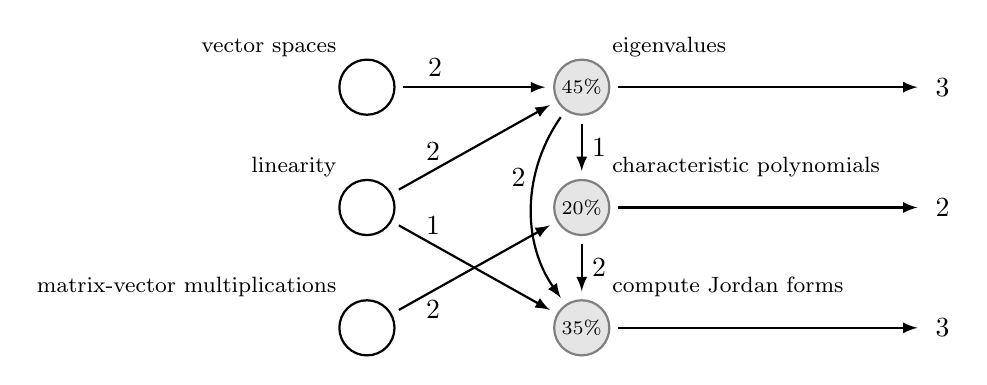
\begin{tikzpicture}
[
	ILO/.style	= {circle, draw = black!50!white, fill = black!10!white, minimum size = 0.7cm, inner sep = 0cm, font = \scriptsize},
	pre/.style	= {ILO, draw = black, fill = white},
	comment/.style	= {font = \footnotesize},
	node distance = 0.8cm and 0.8cm,
	every path/.style = {-latex, thick, shorten < = 0.1cm, shorten > = 0.1cm},
]

	\node (pre1) [pre] {};
	\node (pre2) [pre, below = of pre1] {};
	\node (pre3) [pre, below = of pre2] {};
	%
	\node (ILO1) [ILO, right = 2cm of pre1] {45\%};
	\node (ILO2) [ILO, below = of ILO1] {20\%};
	\node (ILO3) [ILO, below = of ILO2] {35\%};
	%
	\node (aux1) [coordinate, right = 4cm of ILO1] {};
	\node (aux2) [coordinate, right = 4cm of ILO2] {};
	\node (aux3) [coordinate, right = 4cm of ILO3] {};

	\node [comment, above left = 0cm of pre1] {vector spaces};
	\node [comment, above left = 0cm of pre2] {linearity};
	\node [comment, above left = 0cm of pre3] {matrix-vector multiplications};
	%
	\node [comment, above right = 0cm of ILO1] {eigenvalues};
	\node [comment, above right = 0cm of ILO2] {characteristic polynomials};
	\node [comment, above right = 0cm of ILO3] {compute Jordan forms};

	\draw (pre1) -- (ILO1) node [pos = 0.25, above] {2};
	\draw (pre2) -- (ILO1) node [pos = 0.25, above] {2};
	\draw (pre2) -- (ILO3) node [pos = 0.25, above] {1};
	\draw (pre3) -- (ILO2) node [pos = 0.25, below] {2};

	\draw (ILO1) -- (ILO2) node [pos = 0.5, right] {1};
	\draw [out = 235, in = 125] (ILO1) to node [pos = 0.35, left] {2} (ILO3);
	\draw (ILO2) -- (ILO3) node [pos = 0.5, right] {2};

	\draw (ILO1) -- (aux1) node [pos = 1.0, right] {3};
	\draw (ILO2) -- (aux2) node [pos = 1.0, right] {2};
	\draw (ILO3) -- (aux3) node [pos = 1.0, right] {3};


\end{tikzpicture}

	\end{center}
	\note<1-1>{Obviously this table / domain model can be visualized as a directed weighted graph, that we call a course-wide \ac{DMG}. Already here one can see how the structure of the course can be interpreted in terms of "learning flows".}
\end{frame}


\begin{frame}{Program-wide \aclp{DMG}}
	\begin{center}
		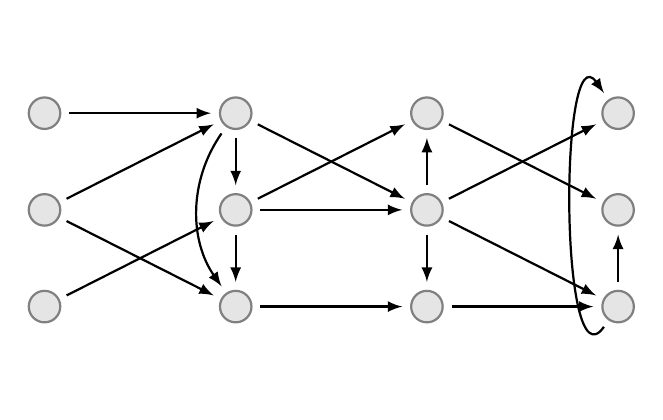
\begin{tikzpicture}
[
% 	transform canvas={scale=0.85},
	ILO/.style	= {circle, draw = black!50!white, fill = black!10!white, minimum size = 0.4cm, inner sep = 0cm, font = \scriptsize},
	pre/.style	= {ILO, draw = black, fill = white},
	comment/.style	= {font = \footnotesize},
	node distance = 0.8cm and 0.6cm,
	every path/.style = {-latex, thick, shorten < = 0.1cm, shorten > = 0.1cm},
]

	\node (pre1) [ILO] {};
	\node (pre2) [ILO, below = of pre1] {};
	\node (pre3) [ILO, below = of pre2] {};
	%
	\node (ILO1) [ILO, right = 2cm of pre1] {};
	\node (ILO2) [ILO, below = of ILO1] {};
	\node (ILO3) [ILO, below = of ILO2] {};
	%
	\node (ILO11) [ILO, right = 2cm of ILO1] {};
	\node (ILO12) [ILO, below = of ILO11] {};
	\node (ILO13) [ILO, below = of ILO12] {};
	%
	\node (ILO21) [ILO, right = 2cm of ILO11] {};
	\node (ILO22) [ILO, below = of ILO21] {};
	\node (ILO23) [ILO, below = of ILO22] {};

	\draw (pre1) -- (ILO1);
	\draw (pre2) -- (ILO1);
	\draw (pre2) -- (ILO3);
	\draw (pre3) -- (ILO2);
	%
	\draw (ILO1) -- (ILO2);
	\draw [out = 235, in = 125] (ILO1) to (ILO3);
	\draw (ILO2) -- (ILO3);

	\draw (ILO1) -- (ILO12);
	\draw (ILO2) -- (ILO11);
	\draw (ILO2) -- (ILO12);
	\draw (ILO3) -- (ILO13);
	%
	\draw (ILO12) -- (ILO11);
% 	\draw [out = 235, in = 125] (ILO11) to (ILO13);
	\draw (ILO12) -- (ILO13);

	\draw (ILO11) -- (ILO22);
	\draw (ILO12) -- (ILO21);
	\draw (ILO12) -- (ILO23);
	\draw (ILO13) -- (ILO23);
	%
% 	\draw (ILO21) -- (ILO22);
	\draw [out = 235, in = 125] (ILO23) to (ILO21);
	\draw (ILO23) -- (ILO22);

\end{tikzpicture}

	\end{center}
	\pause
	Information that is implicitly or explicitly contained in a program-wide \acp{DMG}:
	\begin{itemize}
		\item logical interconnections and overlaps among courses
		\item temporal progression of the learning levels
	\end{itemize}
	\note<1-1>{Assume now that all the teachers of all the courses within a program compile their own course-wide domain models (and thus graphs). Since programs are often designed in a way that the knowledge concepts developed in some courses are prerequisites for other courses, this means that we can combine the single tables / graphs of the single courses into a program-wide table / graph, as here -- and notice that here we omit writing the numbers and the labels of the various knowledge concepts and skills so to keep the drawing simple. This representation is in practice a graphical description of the ``\emph{learning flows}'' that students should ideally follow during their studies. But actually there is much more information in it.}
	\note<2-2>{Indeed, the operation of merging the single graphs / tables into a program-wide graph / table adds information, because it enables to inspect two components that we could not inspect before:
	\begin{itemize}
		\item a logical component, i.e., the fact that courses relate logically, build up knowledge, overlap, etc.;
		\item a temporal component, i.e., the fact that courses tend to be taken at certain specific times and in certain specific orders.
	\end{itemize}
	Thus to the links of the network we implicitly associate two weights: the learning levels and how much time it passes when jumping from one knowledge concept to an other one.}
\end{frame}


\begin{frame}{The usefulness of program-wide \acp{DMG} \\ \quad in detecting program's \emph{logical} flaws}
	\begin{center}
		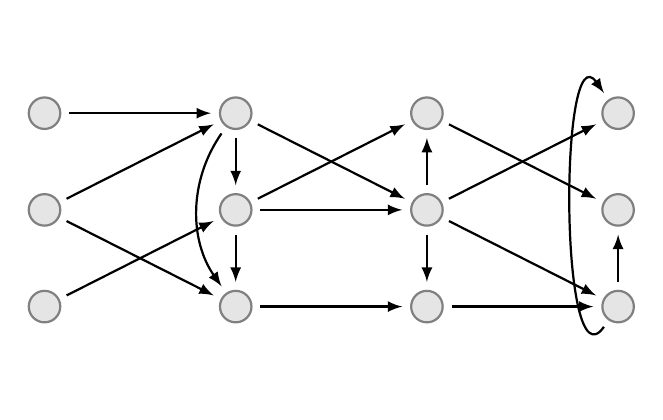
\begin{tikzpicture}
[
% 	transform canvas={scale=0.85},
	ILO/.style	= {circle, draw = black!50!white, fill = black!10!white, minimum size = 0.4cm, inner sep = 0cm, font = \scriptsize},
	pre/.style	= {ILO, draw = black, fill = white},
	comment/.style	= {font = \footnotesize},
	node distance = 0.8cm and 0.6cm,
	every path/.style = {-latex, thick, shorten < = 0.1cm, shorten > = 0.1cm},
]

	\node (pre1) [ILO] {};
	\node (pre2) [ILO, below = of pre1] {};
	\node (pre3) [ILO, below = of pre2] {};
	%
	\node (ILO1) [ILO, right = 2cm of pre1] {};
	\node (ILO2) [ILO, below = of ILO1] {};
	\node (ILO3) [ILO, below = of ILO2] {};
	%
	\node (ILO11) [ILO, right = 2cm of ILO1] {};
	\node (ILO12) [ILO, below = of ILO11] {};
	\node (ILO13) [ILO, below = of ILO12] {};
	%
	\node (ILO21) [ILO, right = 2cm of ILO11] {};
	\node (ILO22) [ILO, below = of ILO21] {};
	\node (ILO23) [ILO, below = of ILO22] {};

	\draw (pre1) -- (ILO1);
	\draw (pre2) -- (ILO1);
	\draw (pre2) -- (ILO3);
	\draw (pre3) -- (ILO2);
	%
	\draw (ILO1) -- (ILO2);
	\draw [out = 235, in = 125] (ILO1) to (ILO3);
	\draw (ILO2) -- (ILO3);

	\draw (ILO1) -- (ILO12);
	\draw (ILO2) -- (ILO11);
	\draw (ILO2) -- (ILO12);
	\draw (ILO3) -- (ILO13);
	%
	\draw (ILO12) -- (ILO11);
% 	\draw [out = 235, in = 125] (ILO11) to (ILO13);
	\draw (ILO12) -- (ILO13);

	\draw (ILO11) -- (ILO22);
	\draw (ILO12) -- (ILO21);
	\draw (ILO12) -- (ILO23);
	\draw (ILO13) -- (ILO23);
	%
% 	\draw (ILO21) -- (ILO22);
	\draw [out = 235, in = 125] (ILO23) to (ILO21);
	\draw (ILO23) -- (ILO22);

\end{tikzpicture}

	\end{center}
	\begin{itemize}
		\item are there ``knowledge jumps''?
	\end{itemize}
	\note<1-1>{Intuitively, it is important to include the knowledge levels progressions because the programs (but also the individual courses) should be designed without having "knowledge jumps". If a course prerequisite is that students have a level knowledge 4 about a certain knowledge concept, then there should be courses that ideally lead students to that level. If the previous courses ideally bring only to level 2, then clearly there is a problem. A PW-DMG can immediately highlight this.}
\end{frame}


\begin{frame}{The usefulness of program-wide \acp{DMG} \\ \quad in detecting program's \emph{temporal} flaws}
	\begin{center}
		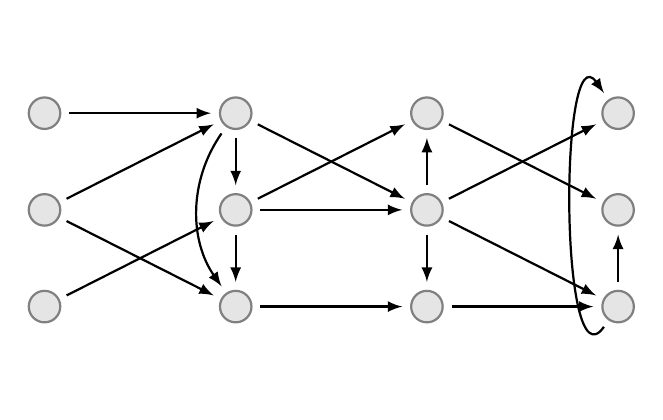
\begin{tikzpicture}
[
% 	transform canvas={scale=0.85},
	ILO/.style	= {circle, draw = black!50!white, fill = black!10!white, minimum size = 0.4cm, inner sep = 0cm, font = \scriptsize},
	pre/.style	= {ILO, draw = black, fill = white},
	comment/.style	= {font = \footnotesize},
	node distance = 0.8cm and 0.6cm,
	every path/.style = {-latex, thick, shorten < = 0.1cm, shorten > = 0.1cm},
]

	\node (pre1) [ILO] {};
	\node (pre2) [ILO, below = of pre1] {};
	\node (pre3) [ILO, below = of pre2] {};
	%
	\node (ILO1) [ILO, right = 2cm of pre1] {};
	\node (ILO2) [ILO, below = of ILO1] {};
	\node (ILO3) [ILO, below = of ILO2] {};
	%
	\node (ILO11) [ILO, right = 2cm of ILO1] {};
	\node (ILO12) [ILO, below = of ILO11] {};
	\node (ILO13) [ILO, below = of ILO12] {};
	%
	\node (ILO21) [ILO, right = 2cm of ILO11] {};
	\node (ILO22) [ILO, below = of ILO21] {};
	\node (ILO23) [ILO, below = of ILO22] {};

	\draw (pre1) -- (ILO1);
	\draw (pre2) -- (ILO1);
	\draw (pre2) -- (ILO3);
	\draw (pre3) -- (ILO2);
	%
	\draw (ILO1) -- (ILO2);
	\draw [out = 235, in = 125] (ILO1) to (ILO3);
	\draw (ILO2) -- (ILO3);

	\draw (ILO1) -- (ILO12);
	\draw (ILO2) -- (ILO11);
	\draw (ILO2) -- (ILO12);
	\draw (ILO3) -- (ILO13);
	%
	\draw (ILO12) -- (ILO11);
% 	\draw [out = 235, in = 125] (ILO11) to (ILO13);
	\draw (ILO12) -- (ILO13);

	\draw (ILO11) -- (ILO22);
	\draw (ILO12) -- (ILO21);
	\draw (ILO12) -- (ILO23);
	\draw (ILO13) -- (ILO23);
	%
% 	\draw (ILO21) -- (ILO22);
	\draw [out = 235, in = 125] (ILO23) to (ILO21);
	\draw (ILO23) -- (ILO22);

\end{tikzpicture}

	\end{center}
	\begin{itemize}
		\item are there ``temporal jumps''?
	\end{itemize}
	\note<1-1>{Intuitively, it is also important to inspect the temporal component because not refreshing a knowledge concept sufficiently often may lead students to forget things. Thus having a temporal component enables to analyze if it typically passes too much time for students to refresh certain knowledge concepts. A PW-DMG can immediately highlight problems in the sense of pedagogically non-ideal temporal flows.}
\end{frame}


\begin{frame}{A non-exhaustive list of usages of program-wide \acp{DMG}}
	\begin{description}
		\item[universities:] ease the implementation of the Bologna agreements
			\vspace{0.5cm} 
		\item[industries:] ease communicating needs to the universities
			\vspace{0.5cm} 
		\item[students:] ease detecting miscommunications
			\vspace{0.5cm} 
		\pause
	\end{description}
	\PrimaryRectangle{all this is the scope of FACE-IT}
	\note<1-1>{Having a PW-DMG may also enable (even if not-so-immediately) to do these things. For example:
	\begin{itemize}
		\item easing the implementation of the Bologna agreements by using these representations as a common language to exchange structural information about local programs across different universities, plus infer their compatibility;
		\item moreover these representation may act as ``communication interfaces'' so that industries can tell universities what are their needs and wishes;
		\item then, an other important thing to notice: up to now we assumed that these tables have been compiled only by teachers. But maybe also students may compile them! Indeed if students compile their own versions, this information would provide insights on the students' perception (and thus favor alignment with teachers and ease the spread of opinions).
	\end{itemize}}
	\note<2-2>{This is the scope of the Erasmus+ project that will start in September 2019. The idea is to create IT tools that can be used for all the purposes described above.}
\end{frame}


\begin{frame}{Fostering Awareness on program Contents in higher Education using IT tools: participants}
	Financed through EU funds:
	\begin{itemize}
		\item NTNU (Norway)
		\item Uppsala University (Sweden)
		\item Otto von Guericke University Magdeburg (Germany)
		\item Université Libre de Bruxelles (Belgium)
		\item University of Padova (Italy)
		\vspace{0.5cm} 
	\end{itemize}
	Financed through own funds:
	\begin{itemize}
		\item Lule{\aa} University of Technology (Sweden)
	\end{itemize}
\end{frame}


\begin{frame}{An other \emph{futuristic} usage of program-wide \acp{DMG}}
	\begin{description}
		\item[everybody:] enable data-driven individual learning
	\end{description}
	\note<1-1>{On top of the things above, PW-DMGs may be -- in our opinion -- a fundamental general tool for introducing quantitative and data-driven strategies for the individualized education of any student, in the sense that we define now.}
\end{frame}


\setbeamercolor{background canvas}{bg=white!80!black}
\begin{frame}
	\centering
	\ItPrimary{\Large towards a data-driven approach to education}
	\note<1-1>{An important thing to notice is that all the information that we described up to now is "a priori", in the sense that up to now we did not involve any "collected measurement", i.e., any result from tests / exams / interrogations / exercises. Somehow, up to now the purposes that we described are independent of how the students are actually performing. We will see now how the DMGs can be ideally useful tools to provide holistic insights on the learning performance of the students.}
\end{frame}
\setbeamercolor{background canvas}{bg=white}


\begin{frame}[t]{Towards a data-driven approach to education}
	{Program-wide \acp{DMG} as random fields}
	\begin{center}
		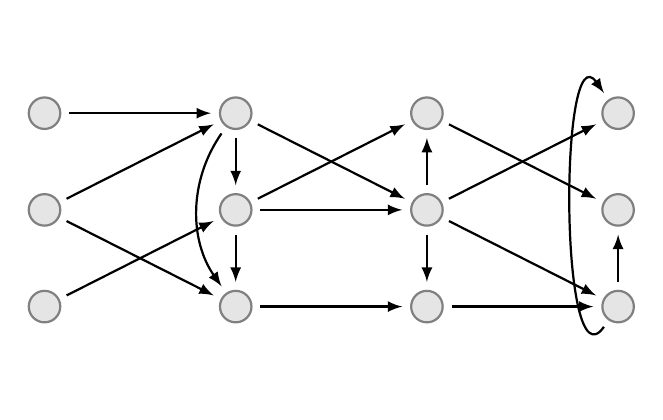
\begin{tikzpicture}
[
% 	transform canvas={scale=0.85},
	ILO/.style	= {circle, draw = black!50!white, fill = black!10!white, minimum size = 0.4cm, inner sep = 0cm, font = \scriptsize},
	pre/.style	= {ILO, draw = black, fill = white},
	comment/.style	= {font = \footnotesize},
	node distance = 0.8cm and 0.6cm,
	every path/.style = {-latex, thick, shorten < = 0.1cm, shorten > = 0.1cm},
]

	\node (pre1) [ILO] {};
	\node (pre2) [ILO, below = of pre1] {};
	\node (pre3) [ILO, below = of pre2] {};
	%
	\node (ILO1) [ILO, right = 2cm of pre1] {};
	\node (ILO2) [ILO, below = of ILO1] {};
	\node (ILO3) [ILO, below = of ILO2] {};
	%
	\node (ILO11) [ILO, right = 2cm of ILO1] {};
	\node (ILO12) [ILO, below = of ILO11] {};
	\node (ILO13) [ILO, below = of ILO12] {};
	%
	\node (ILO21) [ILO, right = 2cm of ILO11] {};
	\node (ILO22) [ILO, below = of ILO21] {};
	\node (ILO23) [ILO, below = of ILO22] {};

	\draw (pre1) -- (ILO1);
	\draw (pre2) -- (ILO1);
	\draw (pre2) -- (ILO3);
	\draw (pre3) -- (ILO2);
	%
	\draw (ILO1) -- (ILO2);
	\draw [out = 235, in = 125] (ILO1) to (ILO3);
	\draw (ILO2) -- (ILO3);

	\draw (ILO1) -- (ILO12);
	\draw (ILO2) -- (ILO11);
	\draw (ILO2) -- (ILO12);
	\draw (ILO3) -- (ILO13);
	%
	\draw (ILO12) -- (ILO11);
% 	\draw [out = 235, in = 125] (ILO11) to (ILO13);
	\draw (ILO12) -- (ILO13);

	\draw (ILO11) -- (ILO22);
	\draw (ILO12) -- (ILO21);
	\draw (ILO12) -- (ILO23);
	\draw (ILO13) -- (ILO23);
	%
% 	\draw (ILO21) -- (ILO22);
	\draw [out = 235, in = 125] (ILO23) to (ILO21);
	\draw (ILO23) -- (ILO22);

\end{tikzpicture}

	\end{center}
	Mathematical interpretation: the \ac{DMG} is a random field $\mathcal{K} : (s, n, t) \mapsto \ell$ 
describing the knowledge level $\ell$ for the generic student $s$ at time $t$ and for the \ac{ILO} $n$
\note<1-1>{Let's start from a numerical interpretation of the DMG. More precisely, the set of ILOs and prerequisites can be thought as the domain of a random field that has, as its codomain, the set of admissible knowledge levels present in the taxonomy that we chose to work with. Informally, the DMG can be seen as a way of summarizing how knowledge levels change in time for the various students. For example, let the node $n = 7$ (i.e., the seventh node in the graph) may be the knowledge concept ``complex numbers'', and the time be $t = 1$ (i.e., first week at the uni). Then if the student $s = \textrm{Ann}$ has a knowledge level 2 for that knowledge concept at that time, we say that $K_{s = \textrm{Ann}} \left( n = 7, t = 1 \right) = 2$. Of course it may be that after 10 weeks of studying, Ann is such that $K_{s = \textrm{Ann}} \left( n = 7, t = 10 \right) = 4$. But she may also forget things in time, so that $K_{s = \textrm{Ann}} \left( n = 7, t = 20 \right) = 3$. If we generalize, we see that $K_{s} \left( n, t \right)$ is a description of how the knowledge for the generic student $s$ changes in time $t$ for the various \acp{ILO} $n$. Note that there exists scientific literature about this topic, that goes under the name of \emph{domain modelling}.}
\end{frame}


\begin{frame}[t]{Towards a data-driven approach to education}
	{The effect of studying}
	\begin{center}
		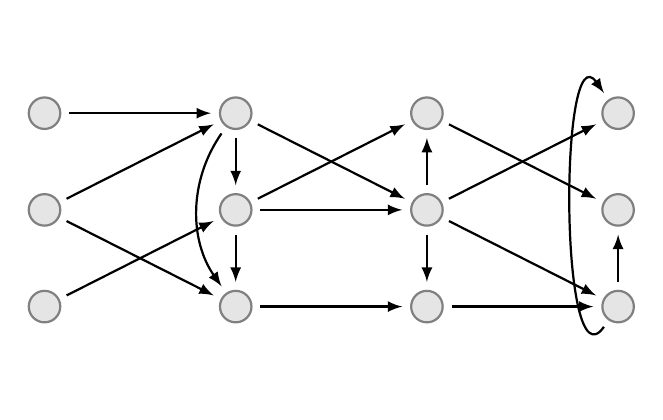
\begin{tikzpicture}
[
% 	transform canvas={scale=0.85},
	ILO/.style	= {circle, draw = black!50!white, fill = black!10!white, minimum size = 0.4cm, inner sep = 0cm, font = \scriptsize},
	pre/.style	= {ILO, draw = black, fill = white},
	comment/.style	= {font = \footnotesize},
	node distance = 0.8cm and 0.6cm,
	every path/.style = {-latex, thick, shorten < = 0.1cm, shorten > = 0.1cm},
]

	\node (pre1) [ILO] {};
	\node (pre2) [ILO, below = of pre1] {};
	\node (pre3) [ILO, below = of pre2] {};
	%
	\node (ILO1) [ILO, right = 2cm of pre1] {};
	\node (ILO2) [ILO, below = of ILO1] {};
	\node (ILO3) [ILO, below = of ILO2] {};
	%
	\node (ILO11) [ILO, right = 2cm of ILO1] {};
	\node (ILO12) [ILO, below = of ILO11] {};
	\node (ILO13) [ILO, below = of ILO12] {};
	%
	\node (ILO21) [ILO, right = 2cm of ILO11] {};
	\node (ILO22) [ILO, below = of ILO21] {};
	\node (ILO23) [ILO, below = of ILO22] {};

	\draw (pre1) -- (ILO1);
	\draw (pre2) -- (ILO1);
	\draw (pre2) -- (ILO3);
	\draw (pre3) -- (ILO2);
	%
	\draw (ILO1) -- (ILO2);
	\draw [out = 235, in = 125] (ILO1) to (ILO3);
	\draw (ILO2) -- (ILO3);

	\draw (ILO1) -- (ILO12);
	\draw (ILO2) -- (ILO11);
	\draw (ILO2) -- (ILO12);
	\draw (ILO3) -- (ILO13);
	%
	\draw (ILO12) -- (ILO11);
% 	\draw [out = 235, in = 125] (ILO11) to (ILO13);
	\draw (ILO12) -- (ILO13);

	\draw (ILO11) -- (ILO22);
	\draw (ILO12) -- (ILO21);
	\draw (ILO12) -- (ILO23);
	\draw (ILO13) -- (ILO23);
	%
% 	\draw (ILO21) -- (ILO22);
	\draw [out = 235, in = 125] (ILO23) to (ILO21);
	\draw (ILO23) -- (ILO22);

\end{tikzpicture}

	\end{center}
	\vspace{-0.5cm} 
	Intuitions:
	\begin{itemize}
		\item student $s$ studies the \ac{KC} $n$ at time $\overline{t}$ $\implies$ $\mathcal{K}_{s} \left( n, t \right)$ increases for $t \geq \overline{t}$
		\item student $s$ doesn't study anymore the \ac{KC} $n$ from time $\overline{t}$ on $\implies$ $\mathcal{K}_{s} \left( n, t \right)$ decreases for $t \geq \overline{t}$
	\end{itemize}
\note<1-1>{Now when a student studies / participates to a lesson / discusses with somebody, she/he is actively affecting the field, in the sense that (hopefully) she/he increments the field somewhere. However a student may forget something, i.e., her/his field may decrement somewhere if she/he is not refreshing the knowledge somehow. Note that there exists some scientific literature also about this topic, that goes under the name of \emph{learner} or \emph{student modelling}.}
\end{frame}


\begin{frame}[t]{First interesting question: how do \acp{KC} correlate from a learning perspective?}
	\begin{center}
		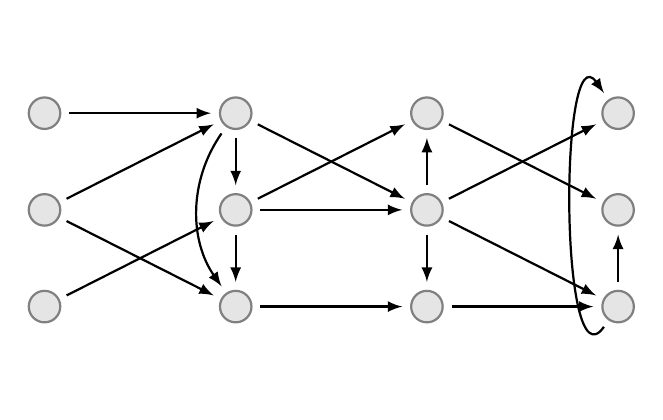
\begin{tikzpicture}
[
% 	transform canvas={scale=0.85},
	ILO/.style	= {circle, draw = black!50!white, fill = black!10!white, minimum size = 0.4cm, inner sep = 0cm, font = \scriptsize},
	pre/.style	= {ILO, draw = black, fill = white},
	comment/.style	= {font = \footnotesize},
	node distance = 0.8cm and 0.6cm,
	every path/.style = {-latex, thick, shorten < = 0.1cm, shorten > = 0.1cm},
]

	\node (pre1) [ILO] {};
	\node (pre2) [ILO, below = of pre1] {};
	\node (pre3) [ILO, below = of pre2] {};
	%
	\node (ILO1) [ILO, right = 2cm of pre1] {};
	\node (ILO2) [ILO, below = of ILO1] {};
	\node (ILO3) [ILO, below = of ILO2] {};
	%
	\node (ILO11) [ILO, right = 2cm of ILO1] {};
	\node (ILO12) [ILO, below = of ILO11] {};
	\node (ILO13) [ILO, below = of ILO12] {};
	%
	\node (ILO21) [ILO, right = 2cm of ILO11] {};
	\node (ILO22) [ILO, below = of ILO21] {};
	\node (ILO23) [ILO, below = of ILO22] {};

	\draw (pre1) -- (ILO1);
	\draw (pre2) -- (ILO1);
	\draw (pre2) -- (ILO3);
	\draw (pre3) -- (ILO2);
	%
	\draw (ILO1) -- (ILO2);
	\draw [out = 235, in = 125] (ILO1) to (ILO3);
	\draw (ILO2) -- (ILO3);

	\draw (ILO1) -- (ILO12);
	\draw (ILO2) -- (ILO11);
	\draw (ILO2) -- (ILO12);
	\draw (ILO3) -- (ILO13);
	%
	\draw (ILO12) -- (ILO11);
% 	\draw [out = 235, in = 125] (ILO11) to (ILO13);
	\draw (ILO12) -- (ILO13);

	\draw (ILO11) -- (ILO22);
	\draw (ILO12) -- (ILO21);
	\draw (ILO12) -- (ILO23);
	\draw (ILO13) -- (ILO23);
	%
% 	\draw (ILO21) -- (ILO22);
	\draw [out = 235, in = 125] (ILO23) to (ILO21);
	\draw (ILO23) -- (ILO22);

\end{tikzpicture}

	\end{center}
	Intuition: increasing the knowledge about $n$ should improve / refresh the knowledge about what leads to $n$
	\note<1-1>{In other words, if I study Fourier transforms, that are defined using complex numbers, then I will likely refresh a bit also complex numbers. Formally, these effects can be cast as a series of probability transitions characterizing the field dynamics, transitions that may be estimated from data -- if we have data. Of course this is a complex problem, since for sure these transitions are affected by a lot of individual socio-psycho-physiological factors. However, the intuition is that the DMG formalism can help getting quantitative models of how learning works in an ``individualized program / individualized person'' perspective. This is the realm of the scientific branches of \emph{adaptive learning} and \emph{intelligent tutoring systems}.}
\end{frame}


\begin{frame}[t]{What is actually a \ac{DMG}?}
	\begin{center}
		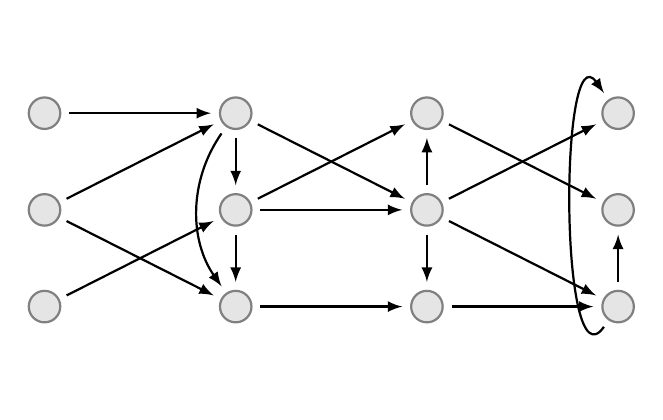
\begin{tikzpicture}
[
% 	transform canvas={scale=0.85},
	ILO/.style	= {circle, draw = black!50!white, fill = black!10!white, minimum size = 0.4cm, inner sep = 0cm, font = \scriptsize},
	pre/.style	= {ILO, draw = black, fill = white},
	comment/.style	= {font = \footnotesize},
	node distance = 0.8cm and 0.6cm,
	every path/.style = {-latex, thick, shorten < = 0.1cm, shorten > = 0.1cm},
]

	\node (pre1) [ILO] {};
	\node (pre2) [ILO, below = of pre1] {};
	\node (pre3) [ILO, below = of pre2] {};
	%
	\node (ILO1) [ILO, right = 2cm of pre1] {};
	\node (ILO2) [ILO, below = of ILO1] {};
	\node (ILO3) [ILO, below = of ILO2] {};
	%
	\node (ILO11) [ILO, right = 2cm of ILO1] {};
	\node (ILO12) [ILO, below = of ILO11] {};
	\node (ILO13) [ILO, below = of ILO12] {};
	%
	\node (ILO21) [ILO, right = 2cm of ILO11] {};
	\node (ILO22) [ILO, below = of ILO21] {};
	\node (ILO23) [ILO, below = of ILO22] {};

	\draw (pre1) -- (ILO1);
	\draw (pre2) -- (ILO1);
	\draw (pre2) -- (ILO3);
	\draw (pre3) -- (ILO2);
	%
	\draw (ILO1) -- (ILO2);
	\draw [out = 235, in = 125] (ILO1) to (ILO3);
	\draw (ILO2) -- (ILO3);

	\draw (ILO1) -- (ILO12);
	\draw (ILO2) -- (ILO11);
	\draw (ILO2) -- (ILO12);
	\draw (ILO3) -- (ILO13);
	%
	\draw (ILO12) -- (ILO11);
% 	\draw [out = 235, in = 125] (ILO11) to (ILO13);
	\draw (ILO12) -- (ILO13);

	\draw (ILO11) -- (ILO22);
	\draw (ILO12) -- (ILO21);
	\draw (ILO12) -- (ILO23);
	\draw (ILO13) -- (ILO23);
	%
% 	\draw (ILO21) -- (ILO22);
	\draw [out = 235, in = 125] (ILO23) to (ILO21);
	\draw (ILO23) -- (ILO22);

\end{tikzpicture}

	\end{center}
	First intuition: if seen as a graph, then it is an educated guess on which causality relations hold among the \acp{KC}
	\note<1-1>{Under the previous light the program flow graph is an educated guess on which causality relations hold among KCs for the average person. In a sense, it is a summary of personal interpretations from the various teachers of which knowledge concepts correlate from a learning perspective, and of how the knowledge levels are supposed to increase in time. This means that a DMG is a prior on the structure of the statistical dependencies among the various scalar variables composing the random field $\mathcal{K}$.}
\end{frame}


\begin{frame}[t]{What is actually a \ac{DMG}?}
	\begin{center}
		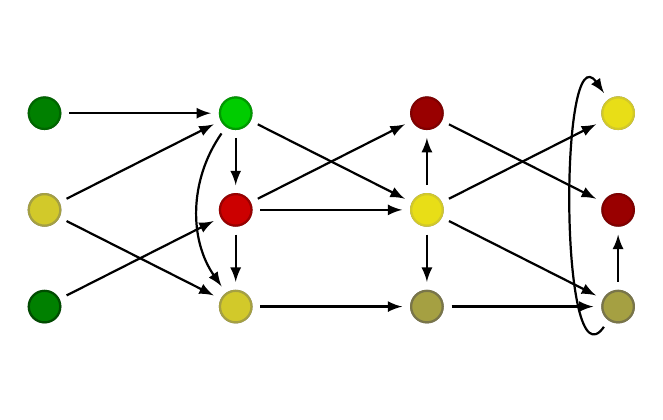
\begin{tikzpicture}
[
% 	transform canvas={scale=0.85},
	ILO/.style	= {circle, draw = black!50!white, fill = black!10!white, minimum size = 0.4cm, inner sep = 0cm, font = \scriptsize},
	pre/.style	= {ILO, draw = black, fill = white},
	comment/.style	= {font = \footnotesize},
	node distance = 0.8cm and 0.6cm,
	every path/.style = {-latex, thick, shorten < = 0.1cm, shorten > = 0.1cm},
]

	\node (pre1) [ILO] {};
	\node (pre2) [ILO, below = of pre1] {};
	\node (pre3) [ILO, below = of pre2] {};
	%
	\node (ILO1) [ILO, right = 2cm of pre1] {};
	\node (ILO2) [ILO, below = of ILO1] {};
	\node (ILO3) [ILO, below = of ILO2] {};
	%
	\node (ILO11) [ILO, right = 2cm of ILO1] {};
	\node (ILO12) [ILO, below = of ILO11] {};
	\node (ILO13) [ILO, below = of ILO12] {};
	%
	\node (ILO21) [ILO, right = 2cm of ILO11] {};
	\node (ILO22) [ILO, below = of ILO21] {};
	\node (ILO23) [ILO, below = of ILO22] {};

	\draw (pre1) -- (ILO1);
	\draw (pre2) -- (ILO1);
	\draw (pre2) -- (ILO3);
	\draw (pre3) -- (ILO2);
	%
	\draw (ILO1) -- (ILO2);
	\draw [out = 235, in = 125] (ILO1) to (ILO3);
	\draw (ILO2) -- (ILO3);

	\draw (ILO1) -- (ILO12);
	\draw (ILO2) -- (ILO11);
	\draw (ILO2) -- (ILO12);
	\draw (ILO3) -- (ILO13);
	%
	\draw (ILO12) -- (ILO11);
% 	\draw [out = 235, in = 125] (ILO11) to (ILO13);
	\draw (ILO12) -- (ILO13);

	\draw (ILO11) -- (ILO22);
	\draw (ILO12) -- (ILO21);
	\draw (ILO12) -- (ILO23);
	\draw (ILO13) -- (ILO23);
	%
% 	\draw (ILO21) -- (ILO22);
	\draw [out = 235, in = 125] (ILO23) to (ILO21);
	\draw (ILO23) -- (ILO22);


	\node at (pre1) [ILO,  draw = green!40!black, fill = green!50!black] {};
	\node at (pre2) [ILO,  draw = yellow!60!black, fill = yellow!80!black] {};
	\node at (pre3) [ILO,  draw = green!30!black, fill = green!50!black] {};
	\node at (ILO1) [ILO,  draw = green!60!black, fill = green!80!black] {};
	\node at (ILO2) [ILO,  draw = red!60!black, fill = red!80!black] {};
	\node at (ILO3) [ILO,  draw = yellow!60!black, fill = yellow!80!black] {};
	\node at (ILO11) [ILO, draw = red!50!black, fill = red!60!black] {};
	\node at (ILO12) [ILO, draw = yellow!80!black, fill = yellow!90!black] {};
	\node at (ILO13) [ILO, draw = yellow!40!black, fill = yellow!60!black] {};
	\node at (ILO21) [ILO, draw = yellow!80!black, fill = yellow!90!black] {};
	\node at (ILO22) [ILO, draw = red!50!black, fill = red!60!black] {};
	\node at (ILO23) [ILO, draw = yellow!40!black, fill = yellow!60!black] {};


\end{tikzpicture}

	\end{center}
	Second intuition: if seen as a function, then it is \ItPrimary{the status of the knowledge of a student about the whole program}
	\note<1-1>{Different persons have not only different learning dynamics: they have also different current ``knowledge state''. Here every node $n$ in the graph has a different color, to indicate a different knowledge level $\ell$ at a specific time, say $t = 10$. This set of levels is a function, in brief $\mathcal{K}_{s = \textrm{Ann}} \left( n, t = 10 \right)$, and it is a summary of what Ann knows 10 weeks after having started her university program about the whole program.}
\end{frame}


\begin{frame}[t]{What is actually an exam?}
	\begin{center}
		\begin{tikzpicture}
[
% 	transform canvas={scale=0.85},
	ILO/.style	= {circle, draw = black!50!white, fill = black!10!white, minimum size = 0.4cm, inner sep = 0cm, font = \scriptsize},
	node distance = 0.8cm and 0.6cm,
	every path/.style = {-latex, thick, shorten < = 0.1cm, shorten > = 0.1cm},
	body/.style = {isosceles triangle, draw, fill = white, shape border rotate = 90, minimum height = 1.1cm},
	head/.style = {circle, draw, fill = white, minimum size = 0.73cm},
	test/.style = {shape = tape, tape bend height = 0.15cm, draw, minimum height = 0.5cm, minimum width = 0.7cm, rotate = 90, tape bend top = out and in, tape bend bottom = out and in, fill = white},
]

	% prior 
	\node (pre1) [ILO] {};
	\node (pre2) [ILO, below = of pre1] {};
	\node (pre3) [ILO, below = of pre2] {};
	%
	\node (ILO1) [ILO, right = 2cm of pre1] {};
	\node (ILO2) [ILO, below = of ILO1] {};
	\node (ILO3) [ILO, below = of ILO2] {};
	%
	\node (ILO11) [ILO, right = 2cm of ILO1] {};
	\node (ILO12) [ILO, below = of ILO11] {};
	\node (ILO13) [ILO, below = of ILO12] {};
	%
	\node (ILO21) [ILO, right = 2cm of ILO11] {};
	\node (ILO22) [ILO, below = of ILO21] {};
	\node (ILO23) [ILO, below = of ILO22] {};

	% paths -- fixed
	\draw (pre1) -- (ILO1);
	\draw (pre2) -- (ILO1);
	\draw (pre2) -- (ILO3);
	\draw (pre3) -- (ILO2);
	%
	\draw (ILO1) -- (ILO2);
	\draw [out = 235, in = 125] (ILO1) to (ILO3);
	\draw (ILO2) -- (ILO3);

	\draw (ILO1) -- (ILO12);
	\draw (ILO2) -- (ILO11);
	\draw (ILO2) -- (ILO12);
	\draw (ILO3) -- (ILO13);
	%
	\draw (ILO12) -- (ILO11);
	\draw (ILO12) -- (ILO13);

	\draw (ILO11) -- (ILO22);
	\draw (ILO12) -- (ILO21);
	\draw (ILO12) -- (ILO23);
	\draw (ILO13) -- (ILO23);
	%
	\draw [out = 235, in = 125] (ILO23) to (ILO21);
	\draw (ILO23) -- (ILO22);

	% student
	\node (PA) [body, yshift = -2cm] at ($(ILO3)!0.5!(ILO13)$) {};
	\node (HA) [head] at (PA.north) {};

	\only<2-2>
	{
		\draw [very thick, dashed, out = 180, in = 270, shorten < = 0.4cm, shorten > = 0.4cm]
		(PA) to node (CX) [pos = 0.5, solid, test] {} (pre3);
		\node [above right = 0.2cm of CX] {exam X};
		%
		\node at (ILO1) [ILO, draw = green!60!black, fill = green!80!black] {};
		\node at (ILO2) [ILO, draw = red!60!black, fill = red!80!black] {};
		\node at (ILO3) [ILO, draw = yellow!60!black, fill = yellow!80!black] {};
	}

	\only<3-3>
	{
		\draw [very thick, dashed, out = 180, in = 270, shorten < = 0.4cm, shorten > = 0.4cm]
		(PA) to node (CY) [pos = 0.5, solid, test] {} (pre3);
		\node [below right = 0.2cm of CY] {exam Y};
		%
		\node at (ILO11) [ILO, draw = red!50!black, fill = red!60!black] {};
		\node at (ILO12) [ILO, draw = yellow!80!black, fill = yellow!90!black] {};
		\node at (ILO13) [ILO, draw = yellow!40!black, fill = yellow!60!black] {};
	}

\end{tikzpicture}

	\end{center}
	Third intuition: any assessable test is a \ItPrimary{noisy and aggregated measurement of the knowledge of a student on part of the program}
	\note<1-1>{Importantly, in this context exams and tests can be seen as operations of sampling from this field: when a student takes an exam, she/he is (noisily) disclosing her knowledge levels relative to some parts of the field to a teacher / device / procedure that performs the assessment, manually or automatically.}
	\note<2-2>{For example, the exam of course X may reveal something about the \acp{ILO} of course X.}
	\note<3-3>{And the same for the exam of course Y. In a sense, every test works in a sense as a "sensor" transforming the state of the system into an output. And even if the current strategies of examining students (and processing of the relative results) are structured in a way that it is unclear how to map an exam / test / exercise into a "measurement" of the various individual variables of the field, however the underlying process can be conceptualized in this way.}
\end{frame}


\begin{frame}[t]{What is actually an exercise?}
	\begin{center}
		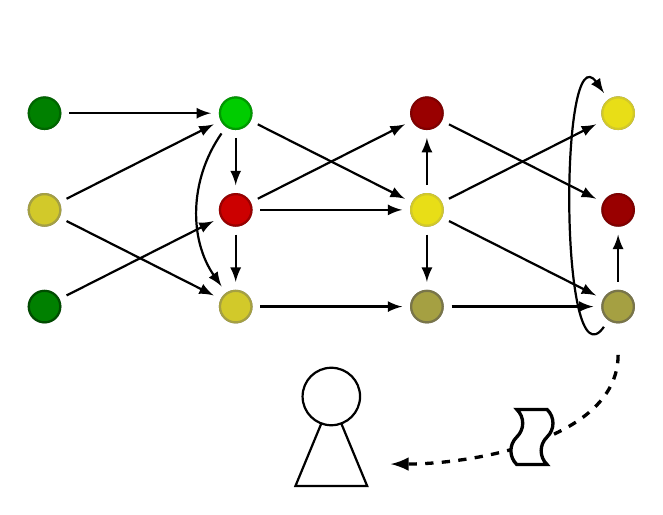
\begin{tikzpicture}
[
% 	transform canvas={scale=0.85},
	ILO/.style	= {circle, draw = black!50!white, fill = black!10!white, minimum size = 0.4cm, inner sep = 0cm, font = \scriptsize},
	node distance = 0.8cm and 0.6cm,
	every path/.style = {-latex, thick, shorten < = 0.1cm, shorten > = 0.1cm},
	body/.style = {isosceles triangle, draw, fill = white, shape border rotate = 90, minimum height = 1.1cm},
	head/.style = {circle, draw, fill = white, minimum size = 0.73cm},
	test/.style = {shape = tape, tape bend height = 0.15cm, draw, minimum height = 0.5cm, minimum width = 0.7cm, rotate = 90, tape bend top = out and in, tape bend bottom = out and in, fill = white},
]

	% prior 
	\node (pre1) [ILO] {};
	\node (pre2) [ILO, below = of pre1] {};
	\node (pre3) [ILO, below = of pre2] {};
	%
	\node (ILO1) [ILO, right = 2cm of pre1] {};
	\node (ILO2) [ILO, below = of ILO1] {};
	\node (ILO3) [ILO, below = of ILO2] {};
	%
	\node (ILO11) [ILO, right = 2cm of ILO1] {};
	\node (ILO12) [ILO, below = of ILO11] {};
	\node (ILO13) [ILO, below = of ILO12] {};
	%
	\node (ILO21) [ILO, right = 2cm of ILO11] {};
	\node (ILO22) [ILO, below = of ILO21] {};
	\node (ILO23) [ILO, below = of ILO22] {};

	% paths -- fixed
	\draw (pre1) -- (ILO1);
	\draw (pre2) -- (ILO1);
	\draw (pre2) -- (ILO3);
	\draw (pre3) -- (ILO2);
	%
	\draw (ILO1) -- (ILO2);
	\draw [out = 235, in = 125] (ILO1) to (ILO3);
	\draw (ILO2) -- (ILO3);

	\draw (ILO1) -- (ILO12);
	\draw (ILO2) -- (ILO11);
	\draw (ILO2) -- (ILO12);
	\draw (ILO3) -- (ILO13);
	%
	\draw (ILO12) -- (ILO11);
	\draw (ILO12) -- (ILO13);

	\draw (ILO11) -- (ILO22);
	\draw (ILO12) -- (ILO21);
	\draw (ILO12) -- (ILO23);
	\draw (ILO13) -- (ILO23);
	%
	\draw [out = 235, in = 125] (ILO23) to (ILO21);
	\draw (ILO23) -- (ILO22);

	% student
	\node (PA) [body, yshift = -2cm] at ($(ILO3)!0.5!(ILO13)$) {};
	\node (HA) [head] at (PA.north) {};

	\draw [very thick, dashed, out = 270, in = 0, shorten < = 0.4cm, shorten > = 0.4cm]
	(ILO23) to node [pos = 0.5, solid, test] {} (PA);
	%
	\node at (pre1) [ILO,  draw = green!40!black, fill = green!50!black] {};
	\node at (pre2) [ILO,  draw = yellow!60!black, fill = yellow!80!black] {};
	\node at (pre3) [ILO,  draw = green!30!black, fill = green!50!black] {};
	\node at (ILO1) [ILO,  draw = green!60!black, fill = green!80!black] {};
	\node at (ILO2) [ILO,  draw = red!60!black, fill = red!80!black] {};
	\node at (ILO3) [ILO,  draw = yellow!60!black, fill = yellow!80!black] {};
	\node at (ILO11) [ILO, draw = red!50!black, fill = red!60!black] {};
	\node at (ILO12) [ILO, draw = yellow!80!black, fill = yellow!90!black] {};
	\node at (ILO13) [ILO, draw = yellow!40!black, fill = yellow!60!black] {};
	\node at (ILO21) [ILO, draw = yellow!80!black, fill = yellow!90!black] {};
	\node at (ILO22) [ILO, draw = red!50!black, fill = red!60!black] {};
	\node at (ILO23) [ILO, draw = yellow!40!black, fill = yellow!60!black] {};

\end{tikzpicture}

	\end{center}
	Fourth intuition: any exercise is a \ItPrimary{indirect push to improve some part of the \ac{DMG}}
	\note<1-1>{Even more importantly, in this context every learning activity that is suggested to the student can be seen as an operation of improving some part of this field.}
\end{frame}


\begin{frame}[t]{Towards learning analytics and intelligent tutoring systems: \\ towards a control-theoretic approach to education}
	LA / ITSs is, in essence, feedback:
	\begin{enumerate}
		\item estimate the current status of the individual student
		\item (if possible) model how that individual student learns
		\item based on the estimated status and learning model, suggest tailored learning activities
	\end{enumerate}
	\note<1-1>{The fact is that with the framework suggested here is the one of the learning analytics / educational data mining communities, that eventually may be interpreted as going towards a control-oriented approach to education: if we know what the student knows and what not, and if we have a model (that shall be intended as a quantitative idea of what will be the effect of doing some specific exercise or generic learning activity), then we can compute what are the ``best'' learning activities (i.e., what to study) that that student should follow. This is what is meant with ``intelligent tutoring systems'', that provide individualized and automatic suggestions to the learners. This is not a new concept, since it has been studied by several authors from the aforementioned \emph{adaptive learning} and \emph{intelligent tutoring systems} communities. However, to the best of our knowledge it has not been studied by people that come from the automatic control community. And we believe that our tools and methods can be very useful to bring improvements in these communities. More specifically, we as automatic control engineers may help with \ldots}
\end{frame}


\begin{frame}[t]{Research topic 1: estimation}
	\begin{center}
		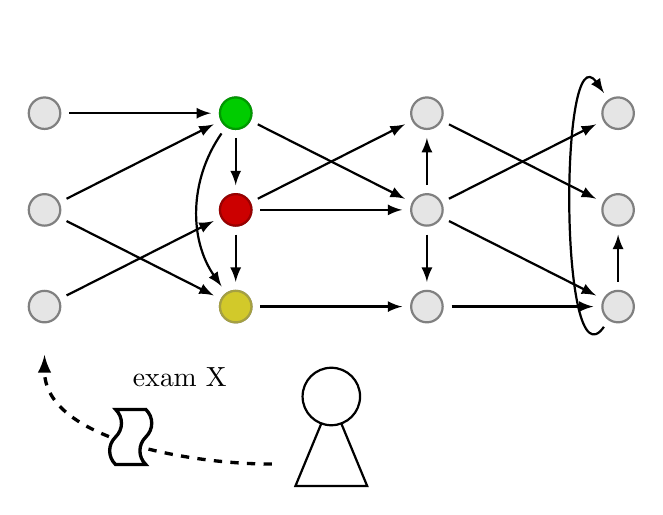
\begin{tikzpicture}
[
% 	transform canvas={scale=0.85},
	ILO/.style	= {circle, draw = black!50!white, fill = black!10!white, minimum size = 0.4cm, inner sep = 0cm, font = \scriptsize},
	node distance = 0.8cm and 0.6cm,
	every path/.style = {-latex, thick, shorten < = 0.1cm, shorten > = 0.1cm},
	body/.style = {isosceles triangle, draw, fill = white, shape border rotate = 90, minimum height = 1.1cm},
	head/.style = {circle, draw, fill = white, minimum size = 0.73cm},
	test/.style = {shape = tape, tape bend height = 0.15cm, draw, minimum height = 0.5cm, minimum width = 0.7cm, rotate = 90, tape bend top = out and in, tape bend bottom = out and in, fill = white},
]

	% prior 
	\node (pre1) [ILO] {};
	\node (pre2) [ILO, below = of pre1] {};
	\node (pre3) [ILO, below = of pre2] {};
	%
	\node (ILO1) [ILO, right = 2cm of pre1] {};
	\node (ILO2) [ILO, below = of ILO1] {};
	\node (ILO3) [ILO, below = of ILO2] {};
	%
	\node (ILO11) [ILO, right = 2cm of ILO1] {};
	\node (ILO12) [ILO, below = of ILO11] {};
	\node (ILO13) [ILO, below = of ILO12] {};
	%
	\node (ILO21) [ILO, right = 2cm of ILO11] {};
	\node (ILO22) [ILO, below = of ILO21] {};
	\node (ILO23) [ILO, below = of ILO22] {};

	% paths -- fixed
	\draw (pre1) -- (ILO1);
	\draw (pre2) -- (ILO1);
	\draw (pre2) -- (ILO3);
	\draw (pre3) -- (ILO2);
	%
	\draw (ILO1) -- (ILO2);
	\draw [out = 235, in = 125] (ILO1) to (ILO3);
	\draw (ILO2) -- (ILO3);

	\draw (ILO1) -- (ILO12);
	\draw (ILO2) -- (ILO11);
	\draw (ILO2) -- (ILO12);
	\draw (ILO3) -- (ILO13);
	%
	\draw (ILO12) -- (ILO11);
	\draw (ILO12) -- (ILO13);

	\draw (ILO11) -- (ILO22);
	\draw (ILO12) -- (ILO21);
	\draw (ILO12) -- (ILO23);
	\draw (ILO13) -- (ILO23);
	%
	\draw [out = 235, in = 125] (ILO23) to (ILO21);
	\draw (ILO23) -- (ILO22);

	% student
	\node (PA) [body, yshift = -2cm] at ($(ILO3)!0.5!(ILO13)$) {};
	\node (HA) [head] at (PA.north) {};

	\draw [very thick, dashed, out = 180, in = 270, shorten < = 0.4cm, shorten > = 0.4cm]
	(PA) to node (CX) [pos = 0.5, solid, test] {} (pre3);
	\node [above right = 0.2cm of CX] {exam X};
	%
	\node at (ILO1) [ILO, draw = green!60!black, fill = green!80!black] {};
	\node at (ILO2) [ILO, draw = red!60!black, fill = red!80!black] {};
	\node at (ILO3) [ILO, draw = yellow!60!black, fill = yellow!80!black] {};

\end{tikzpicture}

	\end{center}
	\ItPrimary{How can we reconstruct the whole $\mathcal{K}_{s} \left( n, t \right)$ from the results of past and current exams and tests?}
	\note<1-1>{To implement the approach above there is the need to develop methodologies and mathematical tools that solve the needs above. The first need is ``estimation''. This means that we need tools to transform the noisy measurements coming from the results of exams and tests into estimates of the current status of the whole field for a specific student.}
\end{frame}


\begin{frame}[t]{Research topic 2: modelling}
	\begin{center}
		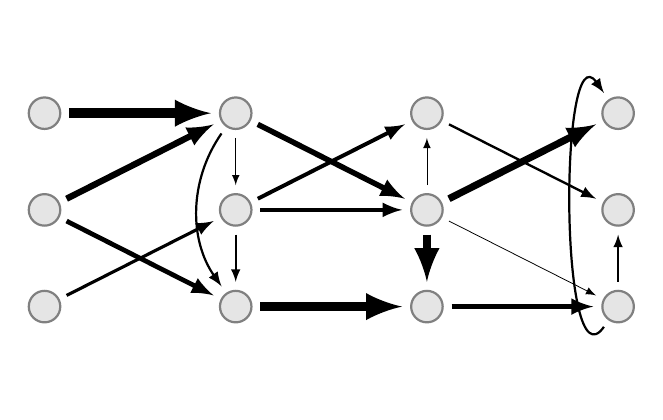
\begin{tikzpicture}
[
% 	transform canvas={scale=0.85},
	ILO/.style	= {circle, draw = black!50!white, fill = black!10!white, minimum size = 0.4cm, inner sep = 0cm, font = \scriptsize},
	pre/.style	= {ILO, draw = black, fill = white},
	comment/.style	= {font = \footnotesize},
	node distance = 0.8cm and 0.6cm,
	every path/.style = {-latex, thick, shorten < = 0.1cm, shorten > = 0.1cm},
]

	\node (pre1) [ILO] {};
	\node (pre2) [ILO, below = of pre1] {};
	\node (pre3) [ILO, below = of pre2] {};
	%
	\node (ILO1) [ILO, right = 2cm of pre1] {};
	\node (ILO2) [ILO, below = of ILO1] {};
	\node (ILO3) [ILO, below = of ILO2] {};
	%
	\node (ILO11) [ILO, right = 2cm of ILO1] {};
	\node (ILO12) [ILO, below = of ILO11] {};
	\node (ILO13) [ILO, below = of ILO12] {};
	%
	\node (ILO21) [ILO, right = 2cm of ILO11] {};
	\node (ILO22) [ILO, below = of ILO21] {};
	\node (ILO23) [ILO, below = of ILO22] {};

	\draw [line width = 0.12cm] (pre1) -- (ILO1);
	\draw [line width = 0.08cm] (pre2) -- (ILO1);
	\draw [line width = 0.06cm] (pre2) -- (ILO3);
	\draw [line width = 0.04cm] (pre3) -- (ILO2);
	%
	\draw [line width = 0.01cm] (ILO1) -- (ILO2);
	\draw [out = 235, in = 125] (ILO1) to (ILO3);
	\draw [line width = 0.02cm] (ILO2) -- (ILO3);

	\draw [line width = 0.07cm] (ILO1) -- (ILO12);
	\draw [line width = 0.05cm] (ILO2) -- (ILO11);
	\draw [line width = 0.05cm] (ILO2) -- (ILO12);
	\draw [line width = 0.12cm] (ILO3) -- (ILO13);
	%
	\draw [line width = 0.01cm] (ILO12) -- (ILO11);
% 	\draw [out = 235, in = 125] (ILO11) to (ILO13);
	\draw [line width = 0.11cm] (ILO12) -- (ILO13);

	\draw [line width = 0.03cm] (ILO11) -- (ILO22);
	\draw [line width = 0.09cm] (ILO12) -- (ILO21);
	\draw [line width = 0.01cm] (ILO12) -- (ILO23);
	\draw [line width = 0.06cm] (ILO13) -- (ILO23);
	%
% 	\draw (ILO21) -- (ILO22);
	\draw [out = 235, in = 125] (ILO23) to (ILO21);
	\draw [line width = 0.02cm] (ILO23) -- (ILO22);

\end{tikzpicture}

	\end{center}
	\ItPrimary{How do we compute the learning model (i.e., the interactions among the variables in $\mathcal{K}_{s} \left( n, t \right)$) of each individual student?}
	\note<1-1>{The second need is ``modelling''. This means that we need tools to transform the noisy measurements coming from the results of exams and tests into estimates of how learning / forgetting a specific topic correlates with learning / forgetting an other topic. In other words, get an individual quantitative (and obviously approximated) description of the learning process. Note that it may be that we obtain only ``average'' models, i.e., not individualized ones, and that they may also be not very accurate descriptions of how these process work.}
\end{frame}


\begin{frame}[t]{Research topic 3: control}
	\begin{center}
		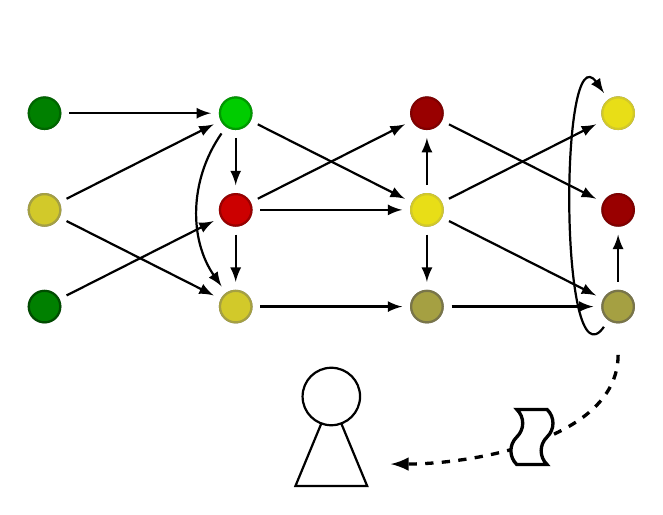
\begin{tikzpicture}
[
% 	transform canvas={scale=0.85},
	ILO/.style	= {circle, draw = black!50!white, fill = black!10!white, minimum size = 0.4cm, inner sep = 0cm, font = \scriptsize},
	node distance = 0.8cm and 0.6cm,
	every path/.style = {-latex, thick, shorten < = 0.1cm, shorten > = 0.1cm},
	body/.style = {isosceles triangle, draw, fill = white, shape border rotate = 90, minimum height = 1.1cm},
	head/.style = {circle, draw, fill = white, minimum size = 0.73cm},
	test/.style = {shape = tape, tape bend height = 0.15cm, draw, minimum height = 0.5cm, minimum width = 0.7cm, rotate = 90, tape bend top = out and in, tape bend bottom = out and in, fill = white},
]

	% prior 
	\node (pre1) [ILO] {};
	\node (pre2) [ILO, below = of pre1] {};
	\node (pre3) [ILO, below = of pre2] {};
	%
	\node (ILO1) [ILO, right = 2cm of pre1] {};
	\node (ILO2) [ILO, below = of ILO1] {};
	\node (ILO3) [ILO, below = of ILO2] {};
	%
	\node (ILO11) [ILO, right = 2cm of ILO1] {};
	\node (ILO12) [ILO, below = of ILO11] {};
	\node (ILO13) [ILO, below = of ILO12] {};
	%
	\node (ILO21) [ILO, right = 2cm of ILO11] {};
	\node (ILO22) [ILO, below = of ILO21] {};
	\node (ILO23) [ILO, below = of ILO22] {};

	% paths -- fixed
	\draw (pre1) -- (ILO1);
	\draw (pre2) -- (ILO1);
	\draw (pre2) -- (ILO3);
	\draw (pre3) -- (ILO2);
	%
	\draw (ILO1) -- (ILO2);
	\draw [out = 235, in = 125] (ILO1) to (ILO3);
	\draw (ILO2) -- (ILO3);

	\draw (ILO1) -- (ILO12);
	\draw (ILO2) -- (ILO11);
	\draw (ILO2) -- (ILO12);
	\draw (ILO3) -- (ILO13);
	%
	\draw (ILO12) -- (ILO11);
	\draw (ILO12) -- (ILO13);

	\draw (ILO11) -- (ILO22);
	\draw (ILO12) -- (ILO21);
	\draw (ILO12) -- (ILO23);
	\draw (ILO13) -- (ILO23);
	%
	\draw [out = 235, in = 125] (ILO23) to (ILO21);
	\draw (ILO23) -- (ILO22);

	% student
	\node (PA) [body, yshift = -2cm] at ($(ILO3)!0.5!(ILO13)$) {};
	\node (HA) [head] at (PA.north) {};

	\draw [very thick, dashed, out = 270, in = 0, shorten < = 0.4cm, shorten > = 0.4cm]
	(ILO23) to node [pos = 0.5, solid, test] {} (PA);
	%
	\node at (pre1) [ILO,  draw = green!40!black, fill = green!50!black] {};
	\node at (pre2) [ILO,  draw = yellow!60!black, fill = yellow!80!black] {};
	\node at (pre3) [ILO,  draw = green!30!black, fill = green!50!black] {};
	\node at (ILO1) [ILO,  draw = green!60!black, fill = green!80!black] {};
	\node at (ILO2) [ILO,  draw = red!60!black, fill = red!80!black] {};
	\node at (ILO3) [ILO,  draw = yellow!60!black, fill = yellow!80!black] {};
	\node at (ILO11) [ILO, draw = red!50!black, fill = red!60!black] {};
	\node at (ILO12) [ILO, draw = yellow!80!black, fill = yellow!90!black] {};
	\node at (ILO13) [ILO, draw = yellow!40!black, fill = yellow!60!black] {};
	\node at (ILO21) [ILO, draw = yellow!80!black, fill = yellow!90!black] {};
	\node at (ILO22) [ILO, draw = red!50!black, fill = red!60!black] {};
	\node at (ILO23) [ILO, draw = yellow!40!black, fill = yellow!60!black] {};

\end{tikzpicture}

	\end{center}
	\ItPrimary{Which current learning activity shall we suggest to each individual student?}
	\note<1-1>{The third need is ``control''. This means that we need tools to transform the uncertain estimates of the current knowledge and uncertain models of how learning activities will affect the current knowledge into learning activities plans. This is a particular instance of the overarching research problem within the realm of automatic control.}
\end{frame}


\begin{frame}[t]{Conclusions}
	\begin{itemize}
		\item program-wide \aclp{DMG} can lead to holistic viewpoints and constructive alignment
		\item \aclp{DMG} can help implementing program-wide learning analytics \ItSecondary{(specially if we add the ``\emph{evaluations from exams}'' ingredient to the picture)}
	\end{itemize}
	\note<1-1>{Summarizing, we foresee that DMGs can lead to these benefits, and that they may help implementing \emph{adaptive learning} and \emph{intelligent tutoring systems} at the university level.}
\end{frame}


% ~~~~~~~~~~~~~~~~~~~~~~~~~~~~~~~~~~~~~~~~~~~~~~~~~~~~~~~~~~~~~~~~~ %
\end{document}														%
% ~~~~~~~~~~~~~~~~~~~~~~~~~~~~~~~~~~~~~~~~~~~~~~~~~~~~~~~~~~~~~~~~~ %


